%!TEX root = ../Master.tex

\section{Localization} % (fold)
\label{sec:localization}

Localization is used when a given robot has no idea of where it is located. The localization tasks consists of two main tasks; sensing and moving. These two tasks are performed alternately as illustrated in \autoref{fig:main tasks}. The robot might have an initial belief of where it is located and in that case this belief is taken into account together with the sense task at first.

\begin{figure}[h]
\centering
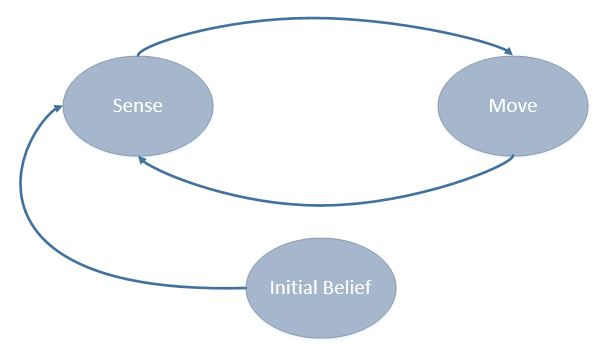
\includegraphics[scale=0.45]{images/SenseMoveInitialBelief}
\caption{Main tasks of localization}
\label{fig:main tasks}
\end{figure}

For the robot to use localization it must be in possession of a map of the environment. The robot uses the map to compare it's belief of it's localization with the map and the results of the sensing.\\

The first of the two tasks for the robot is to sense. This in done by using the sensors which are built in to the robot. For an example the robot could measure the distance to all walls in the environment or the color of the floor. These measurements should lead to a better belief of where the robot is located. Every time the robot senses it gains information of where it is located. The second task for the robot is to move. The robot needs to move in order to be able to get new information from the sensing task. When the robot moves it looses information of where it is located. This is due to inaccuracy of the robots speed and orientation. This will be illustrated in a robot example later on in this section.\\

The algorithm to implement the two tasks is called the Markov Localization algorithm and is illustrated in Algorithm \ref{alg:ml_def1}. The algorithm is based on the Bayes filter algorithm and calculates the new belief based on the old belief $bel(x_{(t-1)})$, the motion $u_t$, the measurements $z_t$ and the map.

% \begin{figure}[H]
% \centering
% 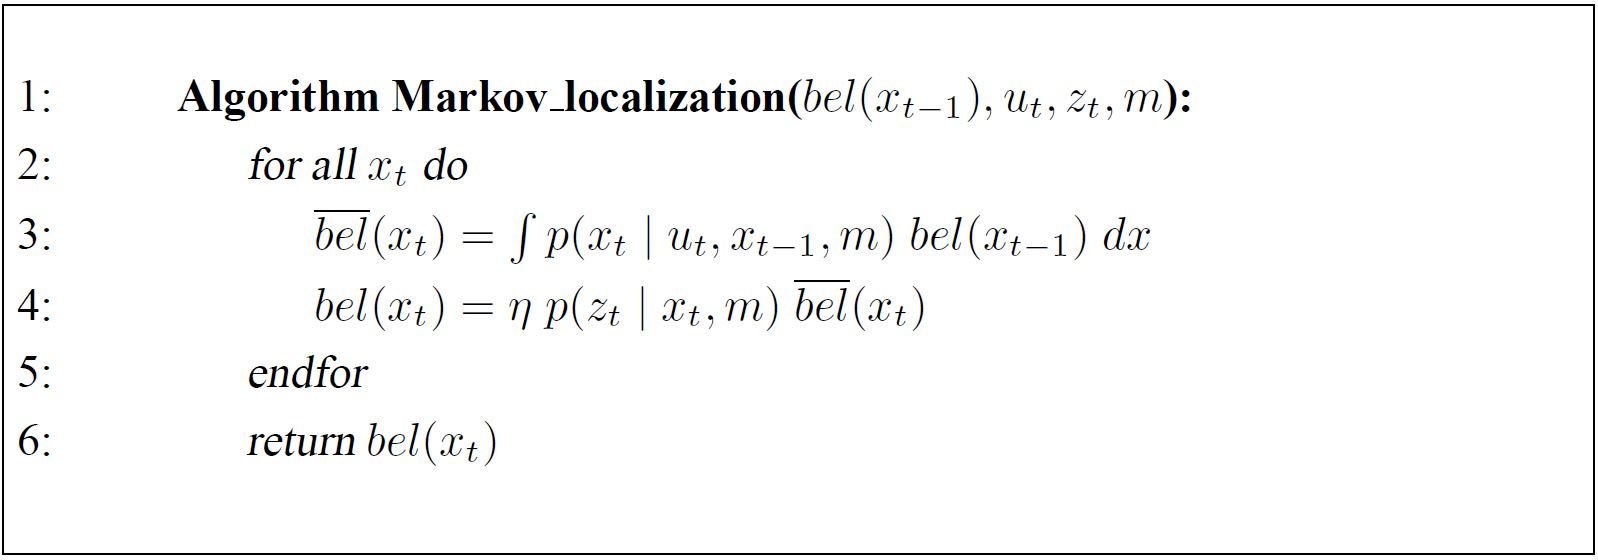
\includegraphics[scale=0.25]{images/MarkovLocalization}
% \caption{The Markov Localization algorithm}
% \label{fig:markovLocalization}
% \end{figure}

\begin{center}
\begin{minipage}{.65\linewidth}
\alglanguage{pseudocode}
\begin{algorithm}[H]
\caption{Markov Localization}
\label{alg:ml_def1}
\begin{algorithmic}[1]
\Procedure{MarkovLocalization}{$bel(x_{t-1}),u_{t},z_{t},m$}
  \ForAll{$x_{t}$}
    \State $\overline{bel}(x_{t}) = \int{p(x_{t}|u_{t},x_{t-1},m)bel(x_{t-1})dx}$
    \State $bel(x_{t}) = \eta\;p(z_{t}|x_{t},m)\overline{bel}(x_{t})$
  \EndFor
  \State \textbf{return} $bel(x_{t})$
\EndProcedure
\end{algorithmic}
\end{algorithm}
\end{minipage}
\end{center}

The first step in the algorithm is line 3 in Algorithm \ref{alg:ml_def1}. In this line the algorithm calculates the sum of the product of two distributions. the two distributions are the prior belief of the robot being at the position $x_{t-1}$ and the probability that the motion $u_t$ moved the robot from the position $x_{t-1}$ to the new position $x_t$ according to the map. This step in the algorithm is referred to as the motion update. \\

The second step is line 4 in Algorithm \ref{alg:ml_def1}. This step looks at the probability that the measurement $z_t$ may have been observed at the the location $x_t$ according to the map. This is multiplied by the belief of $x_t$. This product is normalized by the normalization constant $\eta$ so it will integrate to 1. This step is referred to as the measurement update.\\

The algorithm needs an an prior belief to calculate the new belief. If no initial belief is known the algorithm should use a uniform distribution as the prior belief.

\subsection{Robot Example} % (fold)
\label{sub:robot_example}

This is an example of the localization process where a robot has to localize itself. In \autoref{fig:initialBelief} the scenario is illustrated. The robot is in an environment with three doors. The robot has no idea of where it is located and the initial belief $bel(x)$ is therefore a uniform distribution.

\begin{figure}[H]
\centering
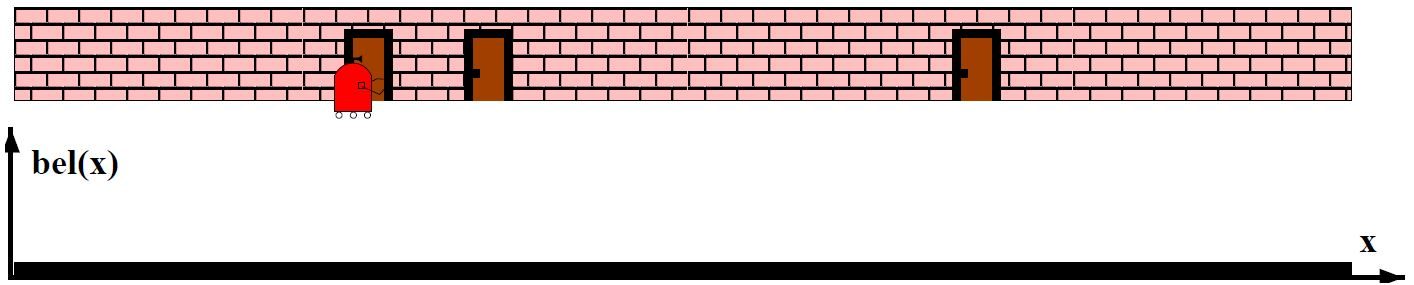
\includegraphics[scale=0.36]{images/MarkovLocalizationA}
\caption{The initial belief of the robot's location}
\label{fig:initialBelief}
\end{figure}

As the robot starts localizing itself is performs a sensing task. The measurement indicates that the robot is localized next to a door. This measurement should only be obtained at three different locations in this environment. The probability of obtaining this measurement when located at those three locations, $p(z|x)$, therefore increases as illustrated in \autoref{fig:afterSenseBelief}. The new belief is calculated as the product of the prior belief and this probability.

\begin{figure}[H]
\centering
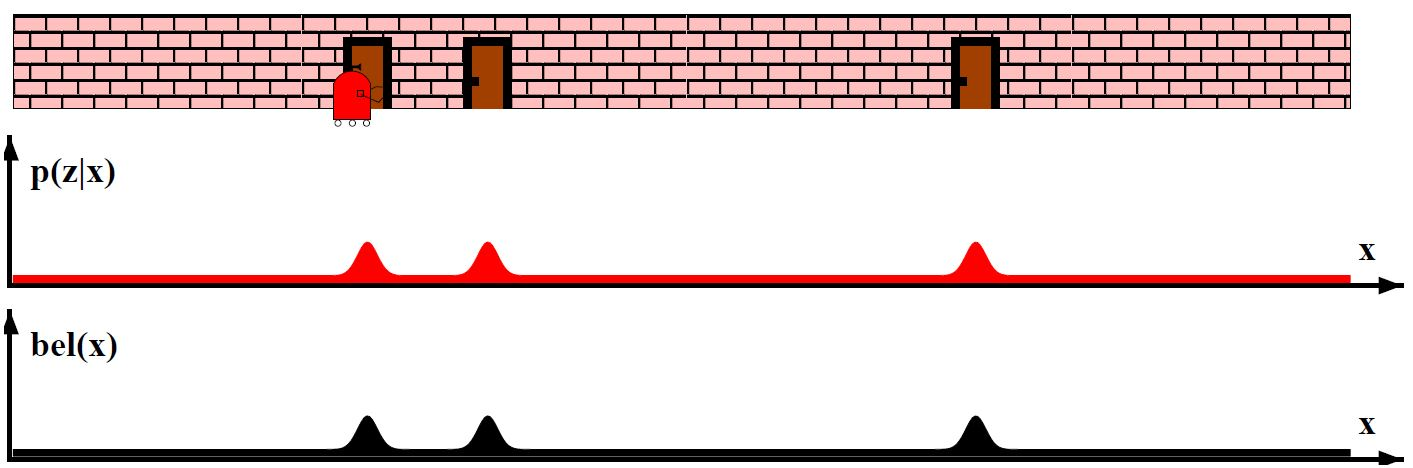
\includegraphics[scale=0.36]{images/MarkovLocalizationB}
\caption{The belief of the robot's location after sensing}
\label{fig:afterSenseBelief}
\end{figure}

The next task for the robot is the moving task. The robot moves a little to the right as illustrated in \autoref{fig:afterMoveBelief}. The belief is now a little less sure of the three most possible locations. This is due to inaccuracy as described earlier in this section.

\begin{figure}[H]
\centering
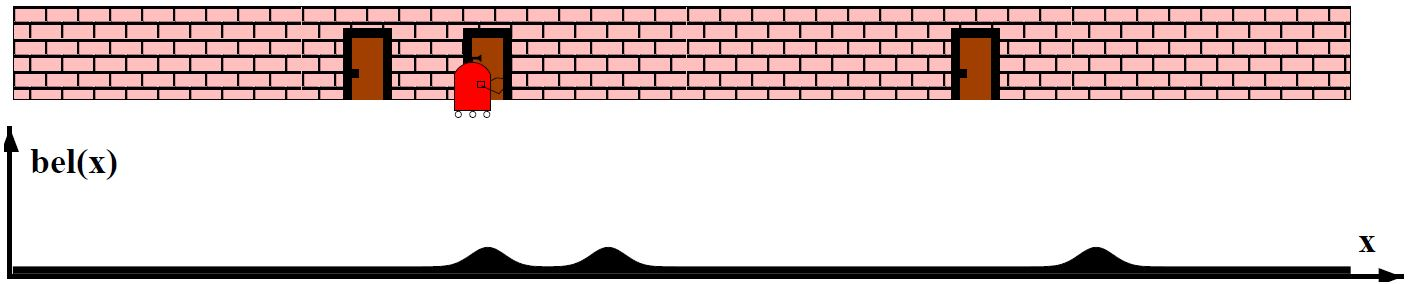
\includegraphics[scale=0.36]{images/MarkovLocalizationC}
\caption{The belief of the robot's location after moving}
\label{fig:afterMoveBelief}
\end{figure}

The robot performs a new sense task and the measurement indicated that the robot is located at a door which leads to a probability similar to the one obtained after the first sensing task. This time, as last time, it is multiplied by the prior belief. This results in a new belief with only one dominant location as illustrated in \autoref{fig:afterSecondSenseBelief}. 

\begin{figure}[H]
\centering
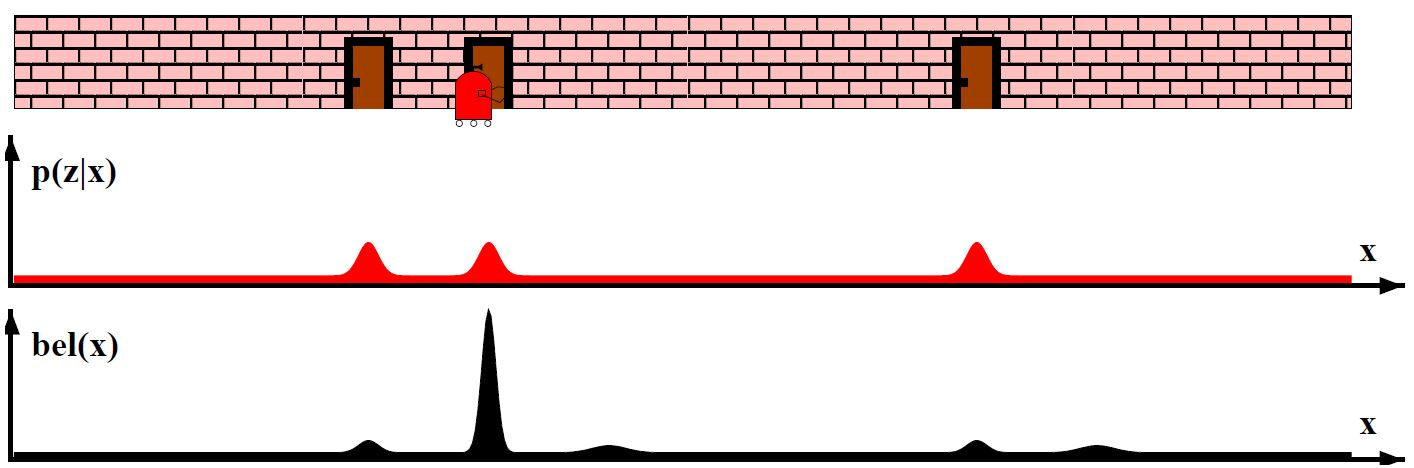
\includegraphics[scale=0.36]{images/MarkovLocalizationD}
\caption{The belief of the robot's location after second sensing}
\label{fig:afterSecondSenseBelief}
\end{figure}

Even though the robot moves the one location is still dominant as illustrated in \autoref{fig:finalBelief}. Hence only one location is dominant he robot has now localized itself.

\begin{figure}[H]
\centering
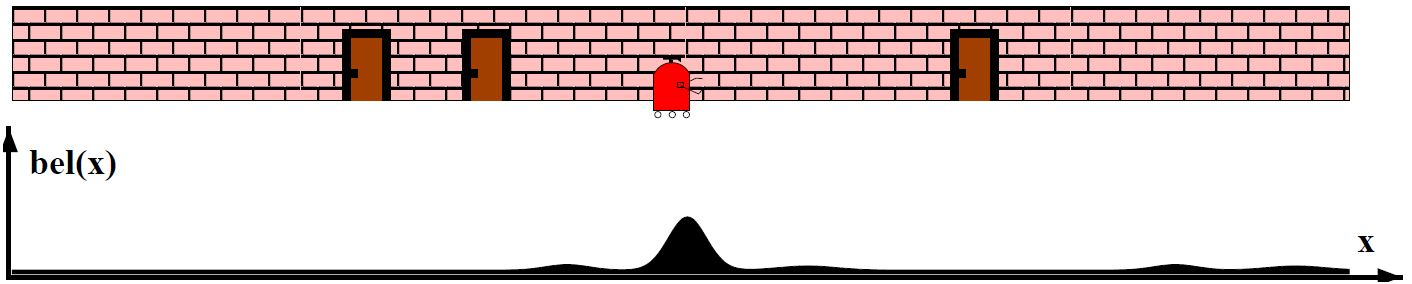
\includegraphics[scale=0.36]{images/MarkovLocalizationE}
\caption{The robot localizes itself}
\label{fig:finalBelief}
\end{figure}

% subsection robot_example (end)

% section localization (end)